


V časti texty, na podstránke indexx.php, nájde užívateľ nadpis a dátum publikácie článkov obr.\ref{OBRAZOK 1.2}. Po kliknutí na nadpis, sa užívateľovi zobrazí len požadovaný článok, ktorý sa rozvinie a zobrazí v celej dĺžke obr.\ref{OBRAZOK 1.3}. Textová/blogová časť kódu a jeho fungovanie bolo inšpirované open-source\footnote[2]{Open-source je zo všeobecného pohľadu akákoľvek informácia, ktorá je dostupná verejnosti bez poplatku(s voľným prístupom), s ohľadom na fakt, že jej voľné šírenie zostane zachované.} projektom\cite{blog}.

\begin{figure}[!tbh]
\centering
\setlength{\fboxsep}{0pt}%
\setlength{\fboxrule}{1pt}%
\fbox{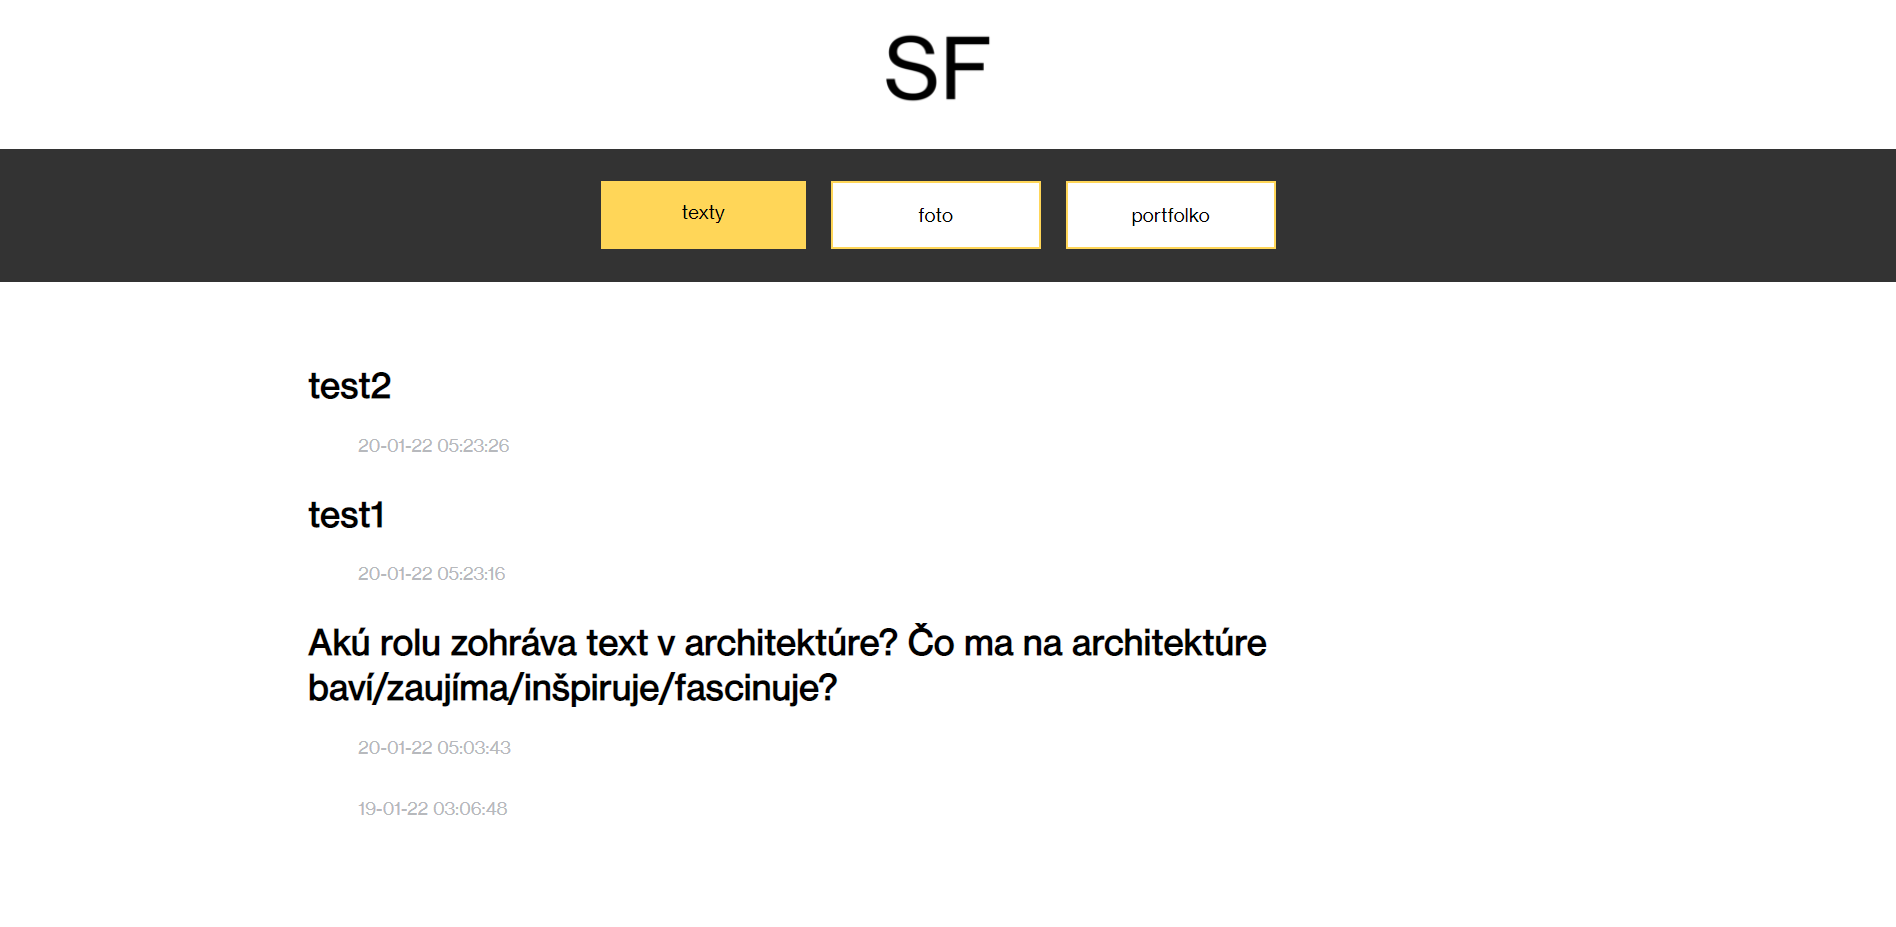
\includegraphics[width=\textwidth]{obr/texty_bez_text.png}}
\caption{Texty publikované na podstránke indexx.php.}\label{OBRAZOK 1.2}
\end{figure}

\begin{figure}[!tbh]
\centering
\setlength{\fboxsep}{0pt}%
\setlength{\fboxrule}{1pt}%
\fbox{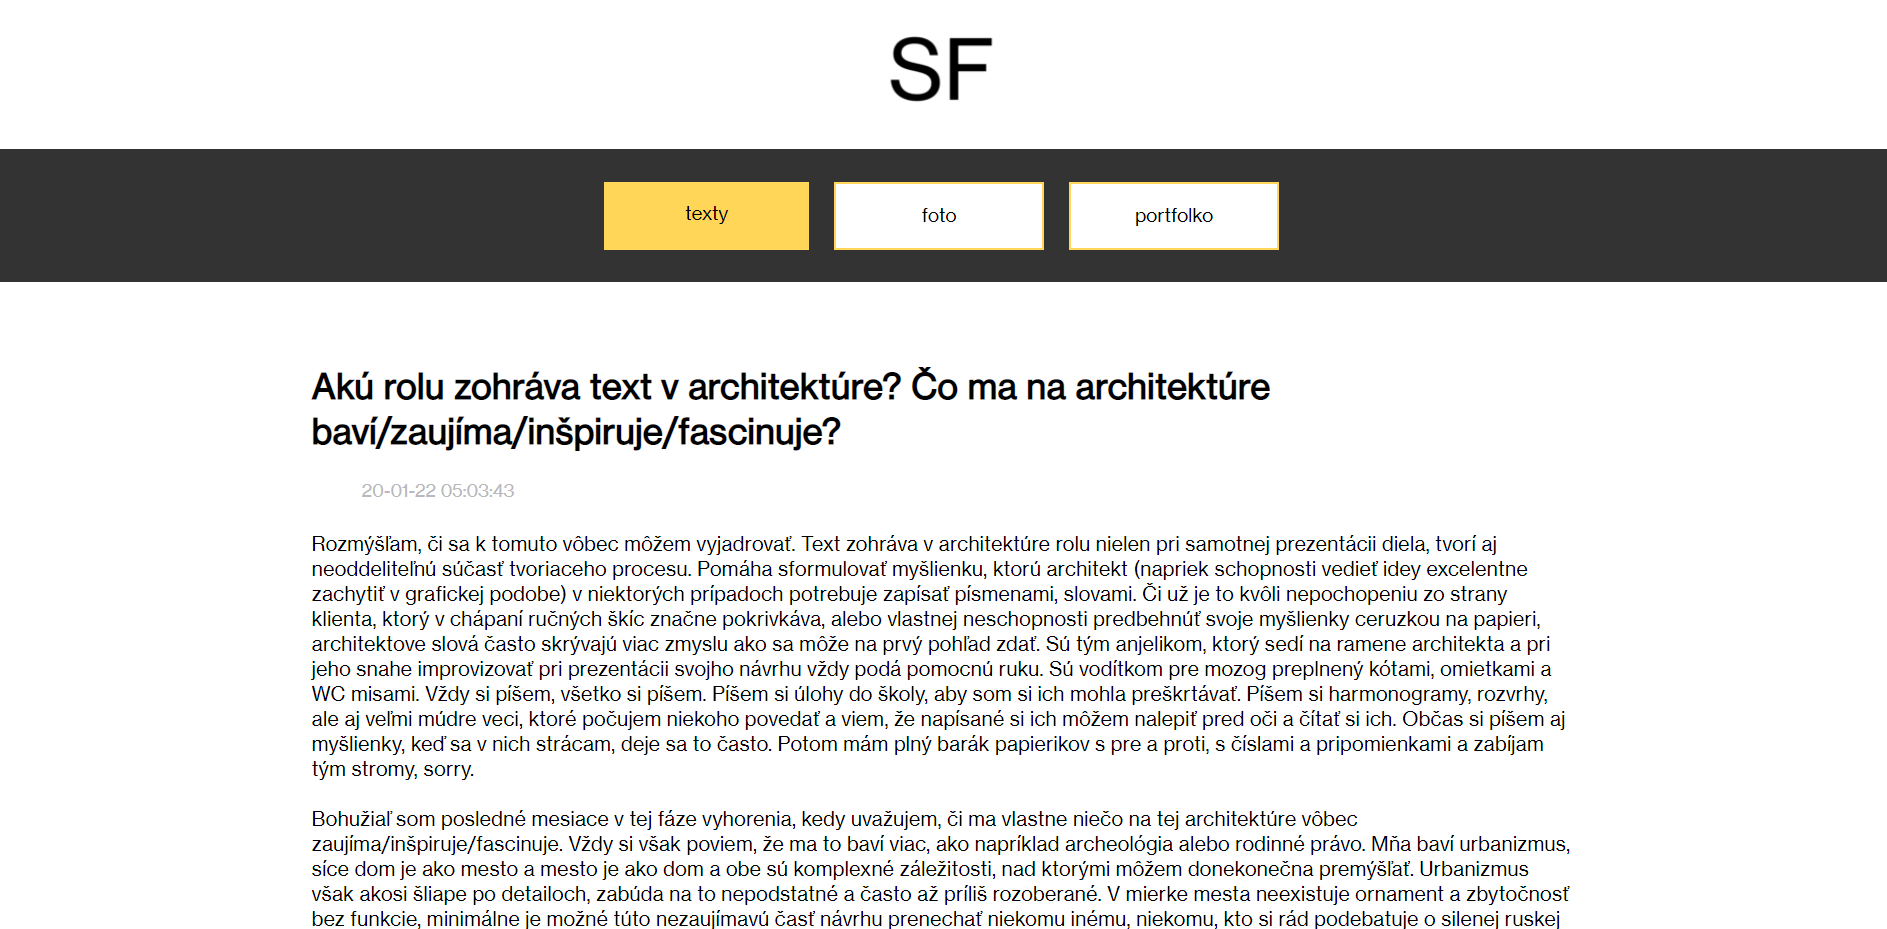
\includegraphics[width=\textwidth]{obr/texty_s_text.png}}
\caption{Zobrazenie konkrétneho textu na podstránke indexx.php.}\label{OBRAZOK 1.3}
\end{figure}

\vspace{5cm}

V časti, foto, nájde užívateľ výber fotiek, ktoré sa klient rozhodol zdieľať obr.\ref{OBRAZOK 1.4}. Fotky sú uložené v radoch, po troch fotkách, a pri prejdení kurzorom nad fotku, sa užívateľovi zobrazí popis fotky obr.\ref{OBRAZOK 1.5}. Pri následnom kliknutí na fotku, sa konkrétna fotka maximalizuje(sú ale určené max. hodnoty šírky) a zobrazí sa aj príslušný nadpis a popis fotky obr.\ref{OBRAZOK 1.6}. Zobrazenie galérie, ako aj fotky v okne, je vykonávané pomocou java script kódu, využitého z open-source projektu\cite{Gallery}.

\begin{figure}[!tbh]
\centering
\setlength{\fboxsep}{0pt}%
\setlength{\fboxrule}{1pt}%
\fbox{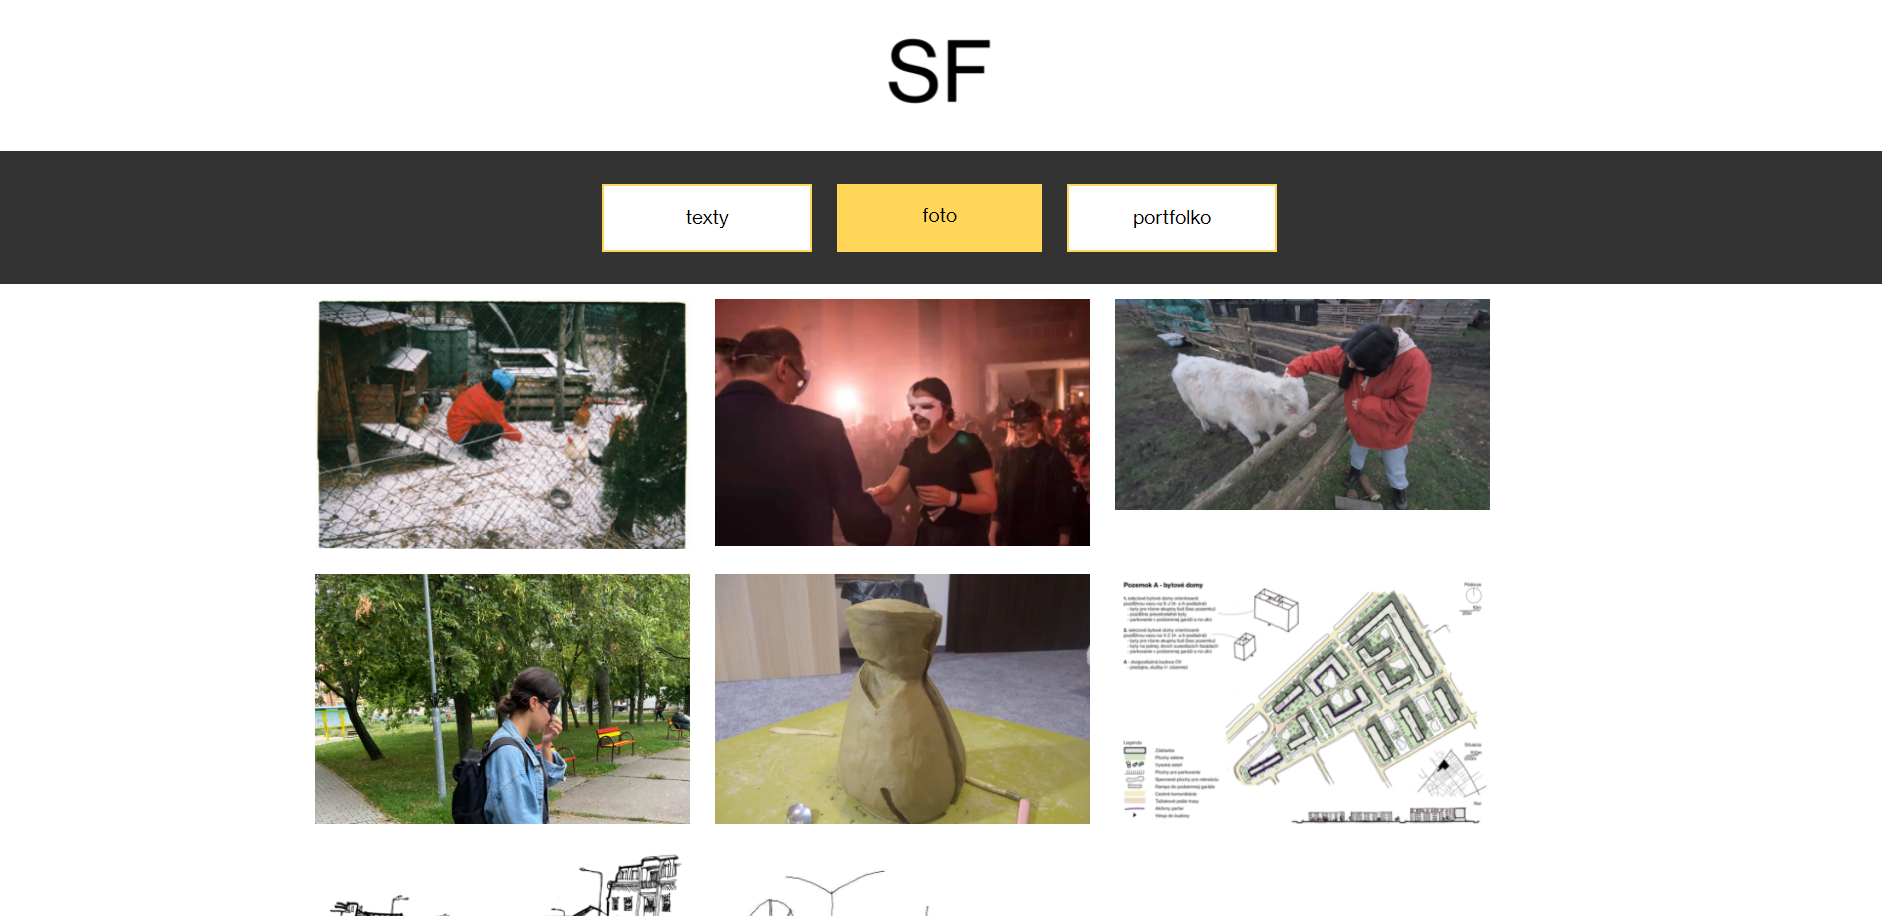
\includegraphics[width=\textwidth]{obr/galeria.png}}
\caption{Fotky publikované na podstránke foto.php.}\label{OBRAZOK 1.4}
\end{figure}

\begin{figure}[!tbh]
\centering
\setlength{\fboxsep}{0pt}%
\setlength{\fboxrule}{1pt}%
\fbox{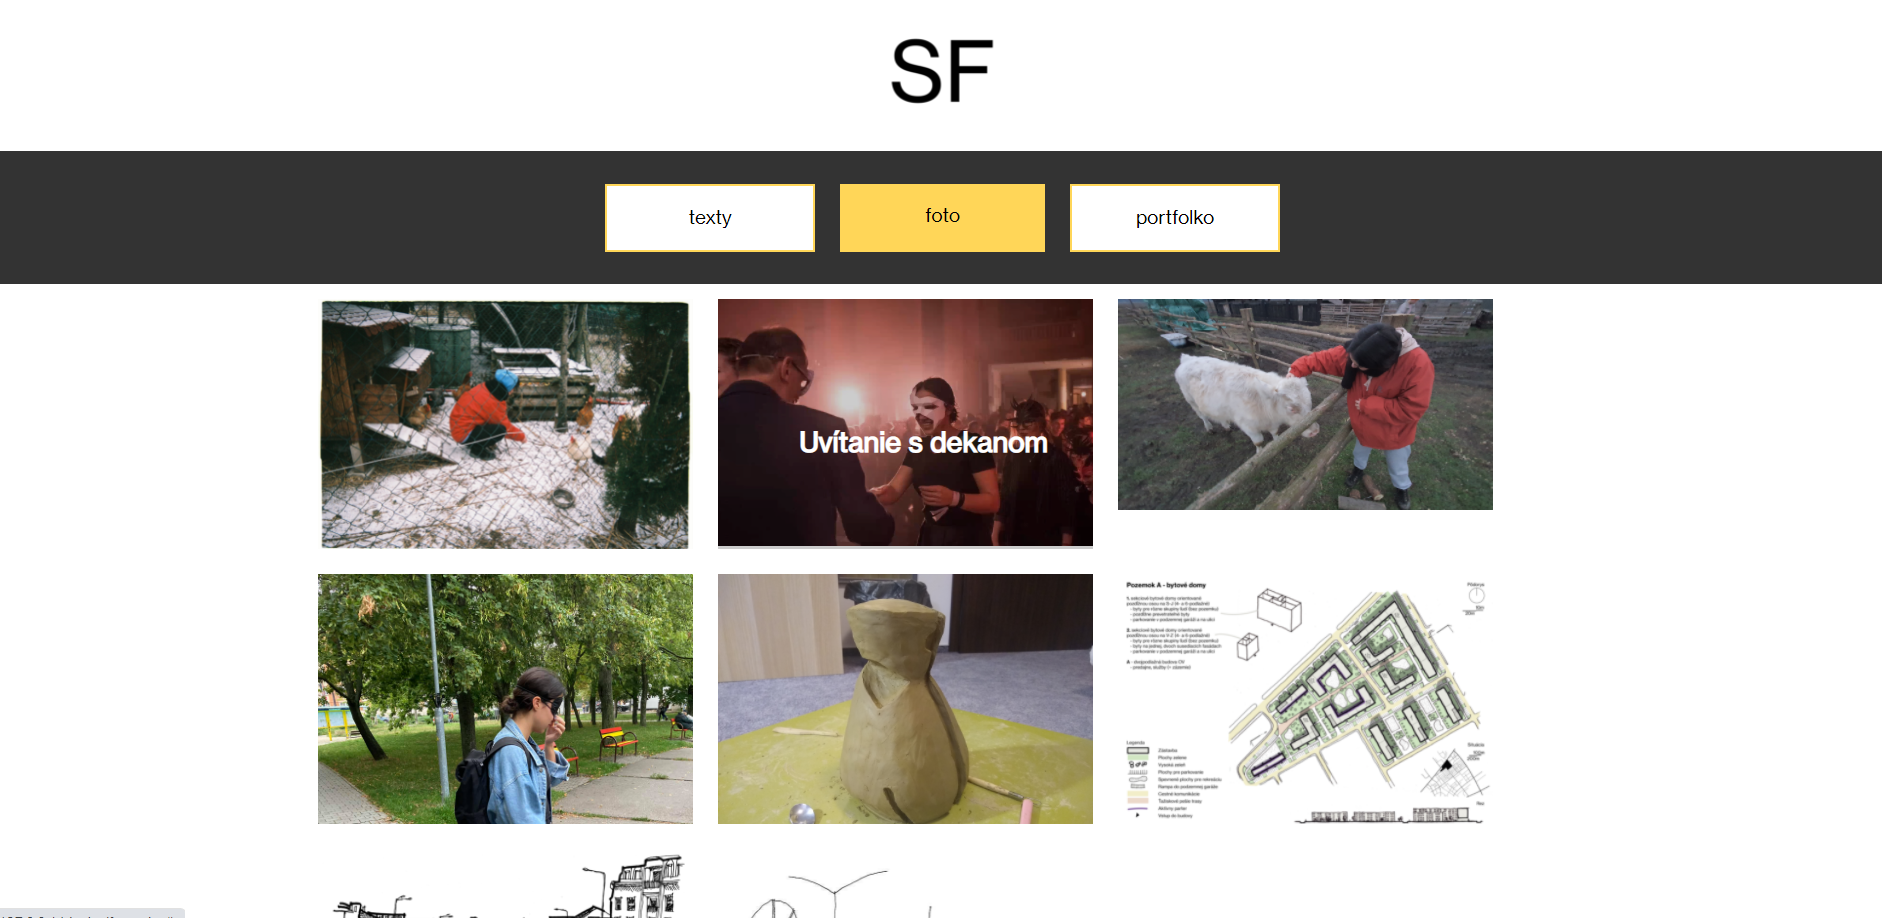
\includegraphics[width=\textwidth]{obr/galeria_nahlad.png}}
\caption{Náhľad popisu fotky na podstránke foto.php.}\label{OBRAZOK 1.5}
\end{figure}

\vspace{2cm}

V časti portfolko, na podstránke portfolio.php, nájde užívateľ jednoduché okno, v ktorom sa zobrazuje PDF súbor portfólia klienta obr.\ref{OBRAZOK 1.7}. Užívateľ si môže PDF súbor prezerať, alebo stiahnuť priamo zo stránky.

\begin{figure}[!tbh]
\centering
\setlength{\fboxsep}{0pt}%
\setlength{\fboxrule}{1pt}%
\fbox{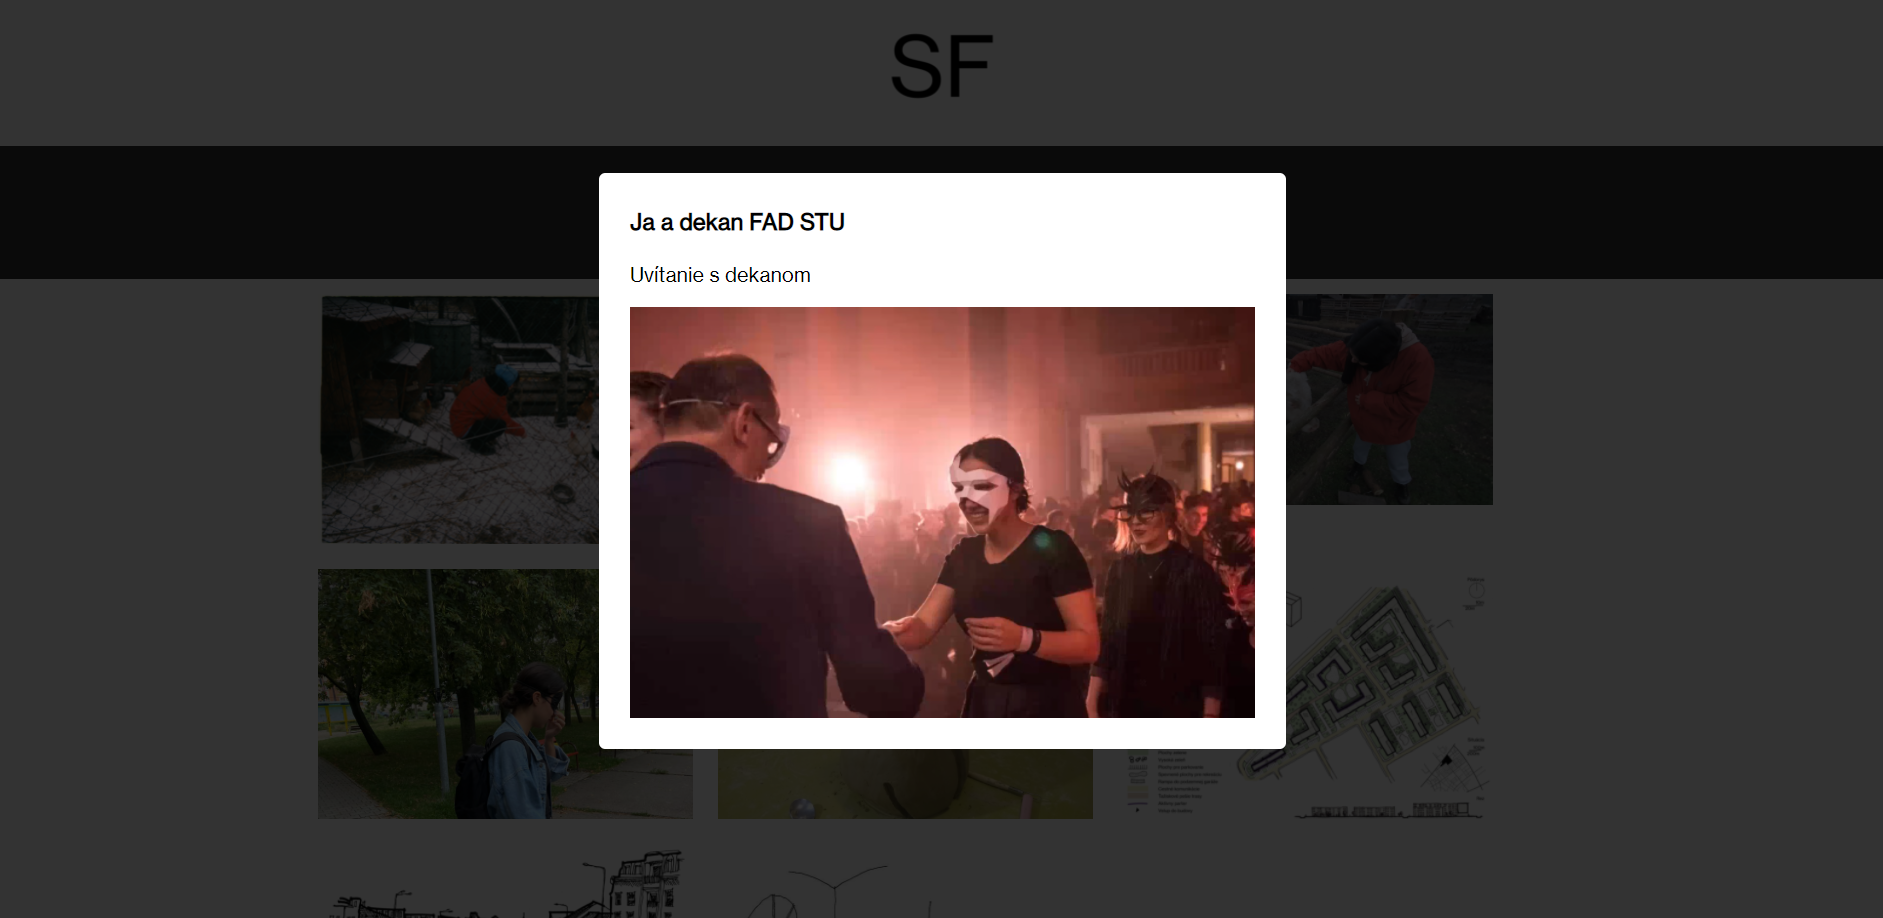
\includegraphics[width=\textwidth]{obr/galeria_zobrazenie.png}}
\caption{Zobrazenie konkrétnej fotky na podstránke foto.php.}\label{OBRAZOK 1.6}
\end{figure}



\begin{figure}[!tbh]
\centering
\setlength{\fboxsep}{0pt}%
\setlength{\fboxrule}{1pt}%
\fbox{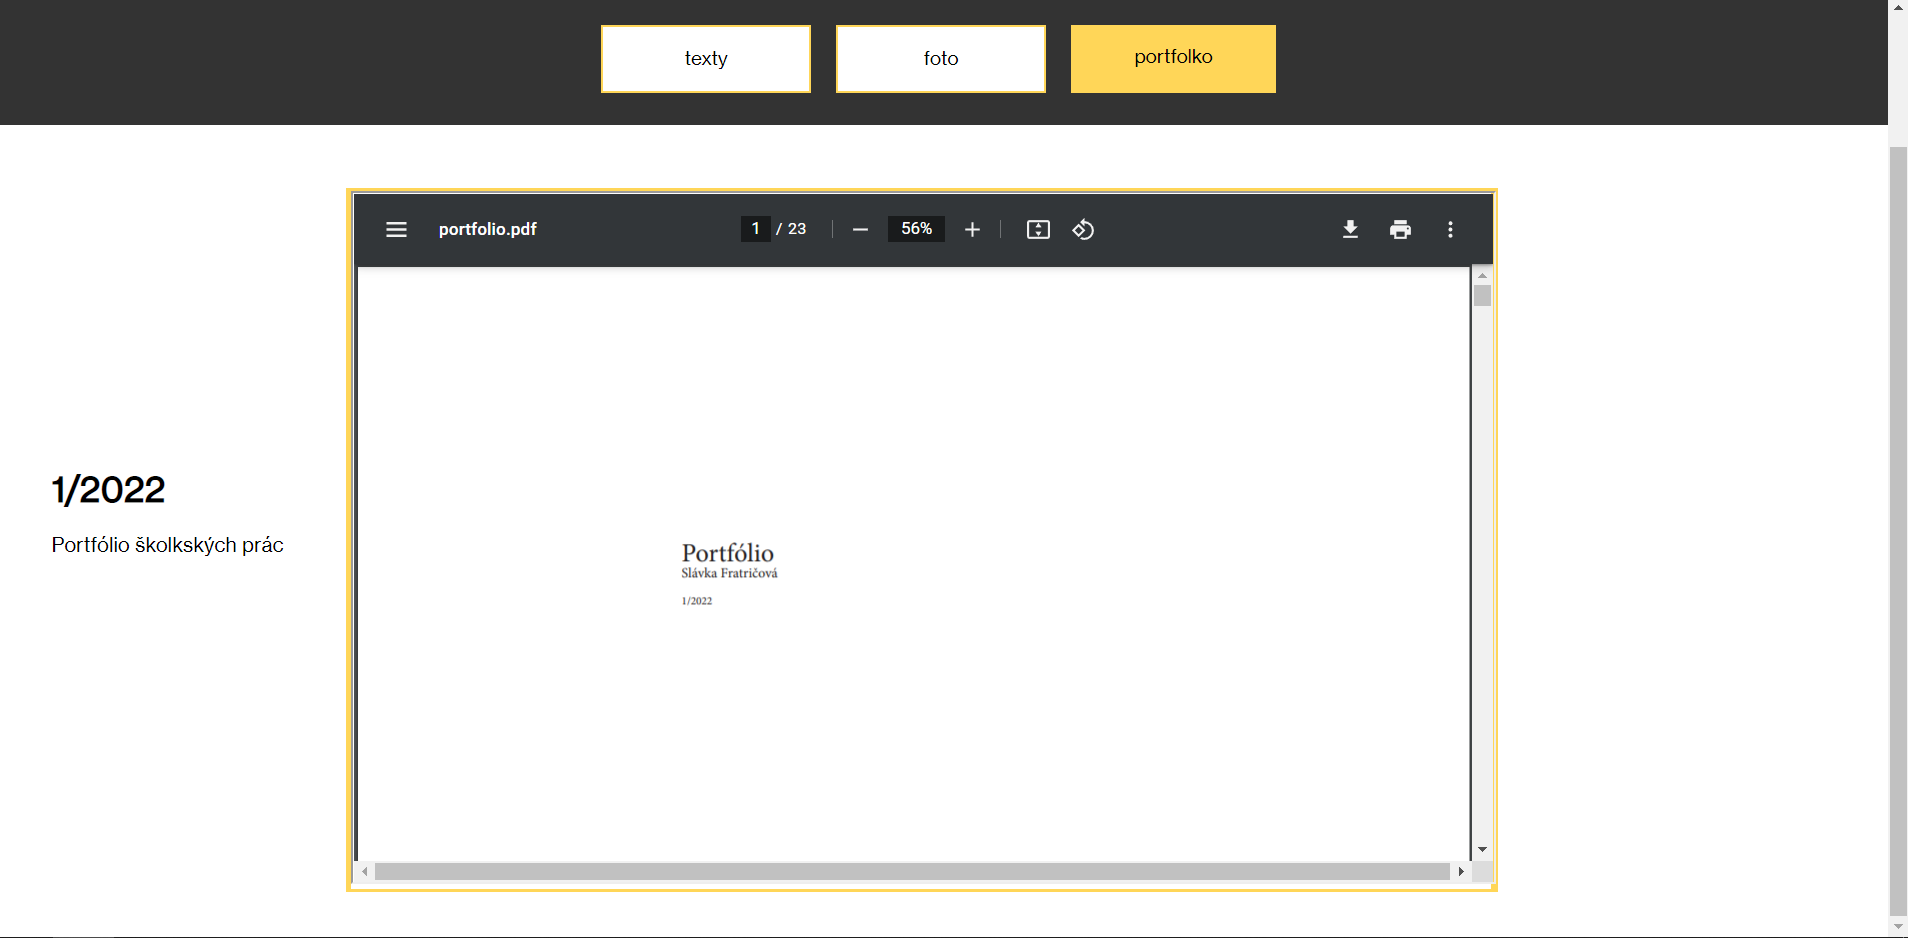
\includegraphics[width=\textwidth]{obr/portfolko.png}}
\caption{Portfólio na podstránke portfolio.php.}\label{OBRAZOK 1.7}
\end{figure}





